%%%%%%%%% Experiments
%
\section{Experiments}
%
\noindent
%
We present experiments to demonstrate that the null-sampled representations are in fact invariant
to $s$ while still allowing a classifier to predict $y$ from them. 
%
We run our \ac{cVAE} and \ac{cFlow} models on the coloured MNIST (cMNIST) and CelebA dataset, which
we artificially bias, first describing the sampling procedure we follow to do so for non-synthetic
datasets. 
%
As baselines we have the model of~\citet{kim2019learning} (Ln2L) and the same \ac{CNN} used to
evaluate the \ac{cFlow} and \ac{cVAE} models but with the unmodified images as input (\acs{CNN}). 
%
For the \ac{cFlow} model we adopt a Glow-like architecture~\citep{KinDha18}, while both
sub-networks of the \ac{cVAE} model comprise gated convolutions~\citep{van2016conditional}, where
the encoding size is \(256\). 
%
For cMNIST, we construct the Ln2L baseline according to its original description, for CelebA, we
treat it as an augmentation of the baseline \ac{CNN}'s objective function.
%More
Detailed information regarding model architectures can be found in \S\ref{sec:architectures} and
\S\ref{sec:nifr-optimisation-details}.
%
\footnote{
    %
    Code can be found at \url{https://github.com/wearepal/nifr}.
    %
}
%
\begin{figure}[tb]
    \centering
    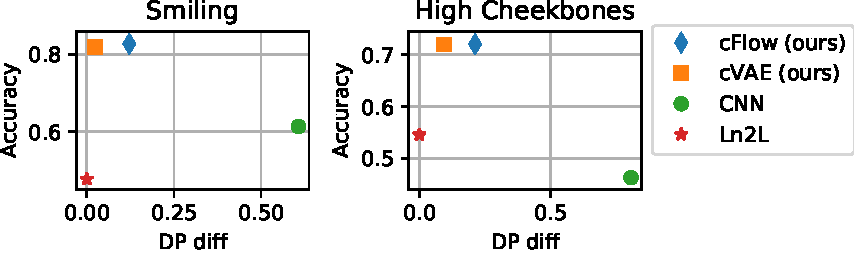
\includegraphics[width=0.7\textwidth]{nifr/Figures/nosinn_celeba.pdf}
    \caption{
        Performance of our model for different targets (mixing factor $\eta=0$).
        Left: \emph{Smiling} as target, right: \emph{high cheekbones}.
        \emph{DP diff} measures fairness with respect to demographic parity.
        A perfectly fair model has a \emph{DP diff} of 0.
    }%
    \label{fig:celeba-targets}
\end{figure}

\begin{figure}[tb]
    \centering
    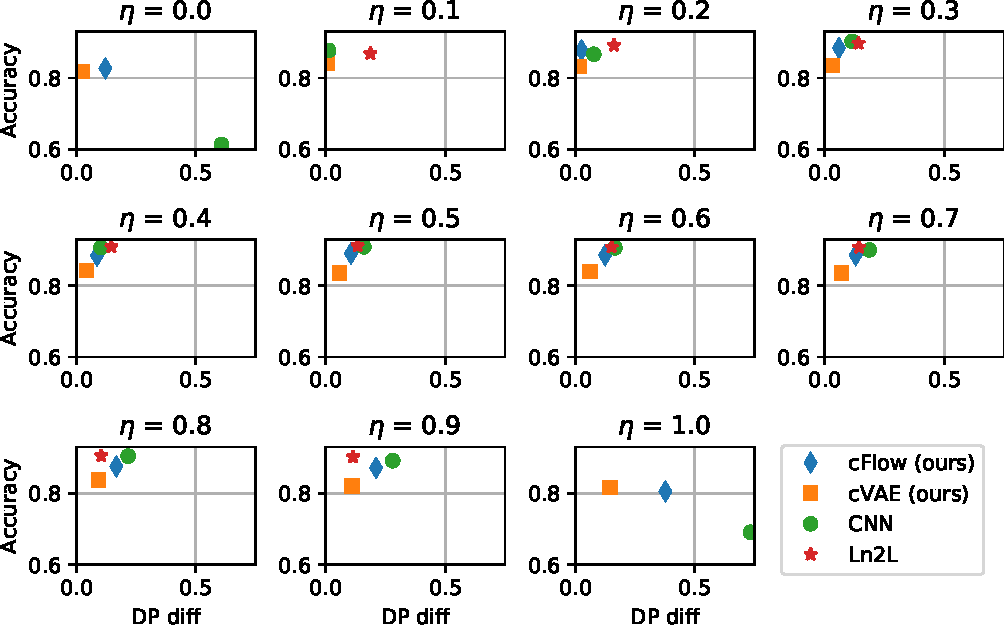
\includegraphics[width=0.85\textwidth]{nifr/Figures/nosinn_celeba_multiplot_all_landscape_Smiling.pdf}
    \caption{
        %
        Performance of our model for the target ``smiling'' for different mixing factors $\eta$.
        %
        \emph{DP diff} measures fairness with respect to demographic parity.
        %
        A perfectly fair model has a \emph{DP diff} of 0, thus the closer to top-left the better it
        is in terms of we accuracy-fairness trade-off.
        %
        Only values $\eta=0$ and $\eta=1$ correspond to the scenario of a strongly biased training
        set.
        %
        The results for $0.1\leq \eta\leq 0.9$ are to confirm that our model does not harm
        performance for non-biased training sets.
    }%
    \label{fig:celeba-multiplot}
\end{figure}
%
\subsection{Synthesising Dataset Bias}
%
For our experiments, we require a training set that exhibits a strong spurious correlation,
together with a test set that does not.
%
For cMNIST, this is easily satisfied as we have complete control over the data generation process.
%
For CelebA and  UCI Adult, on the other hand, we have to generate the split from the existing data.
%
To this end, we first set aside a randomly selected portion of the dataset from which to sample the
biased dataset.
%
The resulting portion is then split further into two parts: one in which \( (s=-1 \land y=-1) \lor
(s=+1 \land y=+1) \) holds true for all samples, call this part \( \mathcal{D}_{eq} \), and the
other part, call it \( \mathcal{D}_{opp} \), which contains the remaining samples.
%
To investigate the behaviour at different levels of correlation, we mix these two subsets according
to a mixing factor \( \eta \).
%
For $\eta \leq \tfrac{1}{2}$, we combine (all of) $\mathcal{D}_{eq}$ with a fraction of $2\eta$
from $\mathcal{D}_{opp}$.
%
For $\eta > \tfrac{1}{2}$, we combine (all of) $\mathcal{D}_{opp}$ and a fraction of $2(1 -\eta)$
from $\mathcal{D}_{eq}$.
%
Thus, for $\eta=0$, the biased dataset is just $\mathcal{D}_{eq}$, for $\eta=1$ it is just
$\mathcal{D}_{opp}$ and for $\eta=\tfrac{1}{2}$ the biased dataset is an ordinary subset of the
whole data. The test set is simply the data remaining from the initial split.
%
\subsection{Evaluation protocol}
%
We evaluate our results in terms of accuracy and fairness. A model that perfectly decouples its
predictions from $s$ will achieve near-uniform accuracy across all biasing-levels. 
%
For binary $s$/$y$ we quantify the fairness of a classifier's predictions using \emph{demographic
parity} (DP): the  absolute difference in the probability  of a positive prediction for each
sensitive group.

\begin{figure}[tb]
    \centering
    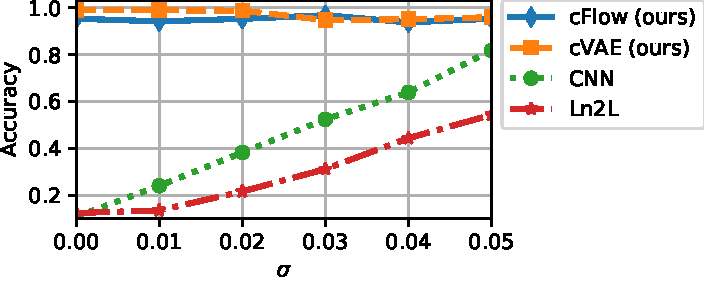
\includegraphics[width=0.7\textwidth]{nifr/Figures/cmnist_new_no_hgr.pdf}
    \caption{
        Accuracy of our approach in comparison with other baseline models on the cMNIST dataset,
        for different standard deviations ($\sigma$) for the colour sampling.
    }%
    \label{fig:cmnist_chart}
\end{figure}

\begin{figure*}[!htb]
    \centering
    \subfloat[Samples from the cMNIST training set, $\sigma=0$.]{%
        \scalebox{0.3}{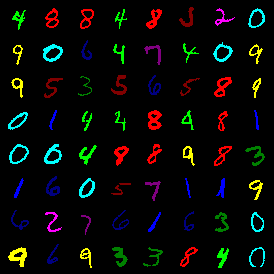
\includegraphics[width=\textwidth]{nifr/Images/cmnist/cflow_original_task_x_scale_0.png}}%
        \label{fig:cflow_cmnist_task_train}
    }
    \hfill
    \subfloat[$x_u$ null-samples from the \ac{cFlow} model.]{%
        \scalebox{0.3}{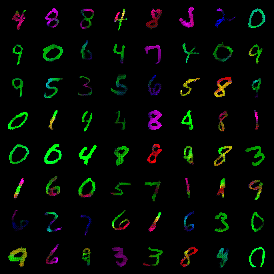
\includegraphics[width=\textwidth]{nifr/Images/cmnist/cflow_task_xy_scale_0.png}}%
        \label{fig:cflow_cmnist_y}
    }
    \hfill
    \subfloat[$x_b$ null-samples from the \ac{cFlow} model.]{%
        \scalebox{0.3}{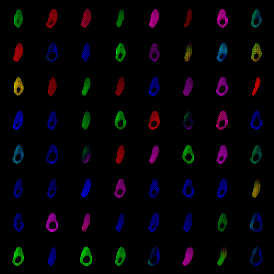
\includegraphics[width=\textwidth]{nifr/Images/cmnist/cflow_task_xs_scale_0.png}}%
        \label{fig:cflow_cmnist_s}
    }
    \caption{
        %
        Sample images from the coloured MNIST dataset problem with $10$ predefined mean colours.
        %
        (a): Images from the spuriously correlated subpopulation where colour is a reliable signal
        of the digit class-label.
        %
        (b-c): Results of running our approach realised with \ac{cFlow} on the cMNIST dataset.
        %
        The model learns to retain the shape of the digit while removing the relationship with
        colour.
        %
        A downstream classifier is now less prone to exploiting correlations between colour and the
        digit label class.
        %
    }\label{fig:cmnist}
\end{figure*}
%
\subsection{Experimental results}
%
We report the results from two image datasets. cMNIST, a synthetic dataset, is a good starting
point for evaluating our model due to the direct control we have over the biasing. 
%
CelebA, on the other hand, is a more practical and challenging example.
%
We also test our method on a tabular dataset, the Adult dataset.
%
\paragraph{cMNIST.}
%
The coloured MNIST (cMNIST) dataset is a variant of the MNIST dataset in which the digits are
coloured.
%
In the training set, the colours have a one-to-one correspondence with the digit class.
%
In the test set (and the representative set), colours are assigned randomly.
%
The colours are drawn from Gaussians with 10 different means.
%
We follow the colourisation procedure outlined by~\citet{kim2019learning}, with the mean colour
values selected so as to be maximally dispersed.
%
The full list of such values can be found in \S\ref{sec:color-details}.
%
We produce multiple variants of the cMNIST dataset corresponding to different standard deviations
$\sigma$ for the colour sampling: $\sigma \in \{0.00, 0.01, ..., 0.05 \}$.

For this specific dataset, we can establish an additional baseline by simply grey-scaling the
dataset which only leaves the luminosity as spurious information.
%
We also evaluate the model, with all the associated hyperparameters, from~\citet{kim2019learning}.
%
The only difference between the setups is the dataset creation, including the range of \(\sigma\)
values we consider.
%
Our versions of the dataset, on the whole, exhibit much stronger colour bias, to the point of the
mapping the digit's colour and class being bijective. 
%
Fig.~\ref{fig:cmnist_chart} shows that the model significantly underperforms even the na\"ive
baseline, aside from at \(\sigma = 0\), where they are at parity.
% CORRECTION: need more explanation of the figures here for me. Maybe can expand now you don't have
% page constraints. In particular comment on whey LN2L does so badly

Inspection of the null-samples shows that both the \ac{cVAE} and \ac{cFlow} model succeed in
removing almost all colour information, which is supported quantitatively by
Fig.~\ref{fig:cmnist_chart}, and qualitatively by Fig.~\ref{fig:cmnist}. 
%
While the \ac{cVAE} outperforms \ac{cFlow} marginally at low \(\sigma\) values, performance degrades
%rapidly
as this increases. 
%
This highlights the problems with the conditional decoder we anticipated in \S\ref{conddec}. 
%
The lower $\sigma$, and therefore the variation in sampled colour, is, the more reliably the $s$
label, corresponding to the mean of RGB distribution, encodes information about the colour. 
%
For higher $\sigma$ values, the sampled colours can deviate far from the mean and so the encoder
must incorporate information about $s$ into its representation if it is to minimise the
reconstruction loss. \ac{cFlow}, on the other hand, is consistent across $\sigma$ values.
%
\paragraph{CelebA.}
%
To evaluate the effectiveness of our framework on real-world image data we use the CelebA
dataset~\citep{liu2015faceattributes}, consisting of 202,599 celebrity images. 
%
These images are annotated with various binary physical  attributes, including ``gender'', ``hair
colour'', ``young'', etc., from which we select our sensitive and target attributes. 
%
The images are centre cropped and resized to $64\times64$, as is standard practice. 
%
For our experiments, we designate ``gender'' as the sensitive attribute, and ``smiling'' and ``high
cheekbones'' as target attributes. 
%
We chose gender as the sensitive attribute as it a common sensitive attribute in the fairness
literature. 
%
For the target attributes, we chose attributes that are harder to learn than gender and which do
not correlate too strongly with gender in the dataset (``wearing lipstick'' for example being an
attribute too closely correlated with gender).
%
The model is trained on the representative set (normal subset of CelebA) and is then used to encode
the artificially biased training set and the test set. The results for the most strongly biased
training set ($\eta=0$) can be found in Fig.~\ref{fig:celeba-targets}. Our method outperforms the
baselines in accuracy and fairness.

\begin{figure*}[tb]
  \centering
  \subfloat[Original images.]{%
      \scalebox{0.3}{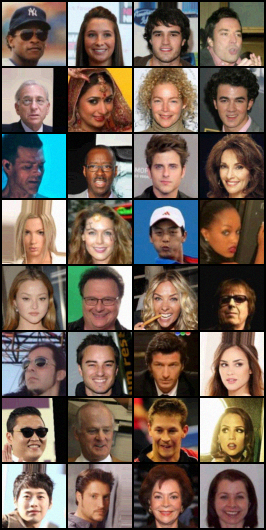
\includegraphics[width=\textwidth]{nifr/Images/celeba/train_original_x_2.png}}%
      \label{fig:cflow_celeba_original_x}
  }
  \hfill
  \subfloat[$\bm{x}_u$ null-samples from the cFlow model.]{%
      \scalebox{0.3}{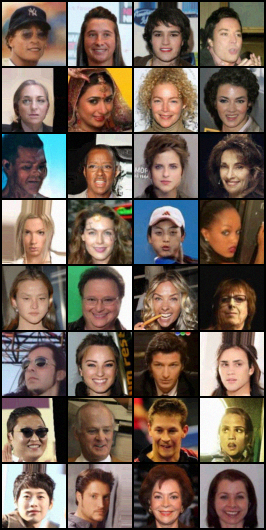
\includegraphics[width=\textwidth]{nifr/Images/celeba/train_reconstruction_y_2.png}}%
      \label{fig:cflow_celeba_recon_y}
  }
  \hfill
  \subfloat[$\bm{x}_b$ null-samples from the cFlow model.]{%
      \scalebox{0.3}{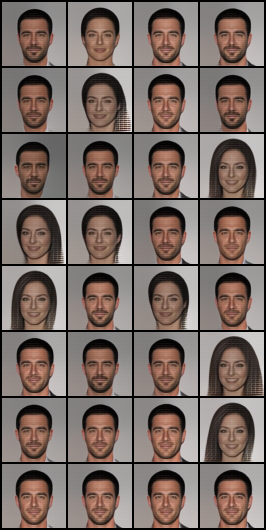
\includegraphics[width=\textwidth]{nifr/Images/celeba/train_reconstruction_s_2.png}}%
      \label{fig:cflow_celeba_recon_s}
  }
  \caption{
      CelebA null-samples learned by our \ac{cFlow} model, with gender as the sensitive attribute.
      %
      (a) The original, untransformed samples from the CelebA dataset
    %
      (b) Reconstructions using only information unrelated to $s$.
    %
      (c) Reconstruction using only information related to $\neg s$.
    %
      The model learns to disentangle gender from the non-gender related information.
      %
      Note that some attributes like skin tone seem to change along with gender due to the
      correlation between the attributes.
    %
      This is especially visible in images (1,1) and (3,2). Only because our representations are
      produced in the data-domain can we easily spot such instances of entanglement.
  }%
  \label{fig:celeba_cflow}
\end{figure*}
%
We also assess performance for different mixing factors ($\eta$) which correspond to varying
degrees of bias in the training set (see Fig.~\ref{fig:celeba-multiplot}).
%
This is to verify that the model does not \emph{harm} performance when there is not much bias in
the training set.
%
For these experiments, the model is trained once on the representative set and is then used to
encode different training sets.
%
The results show that for the intermediate values of $\eta$, our model incurs a small penalty in
terms of accuracy, but at the same time makes the results \emph{fairer} (corresponding to an
accuracy-fairness trade-off). 
%
Qualitative results can be found in Fig.~\ref{fig:celeba_cflow} (images from \ac{cVAE} can be found
in \S\ref{sec:qual-results-celeba}).

To show that our method can handle multinomial, as well as binary, sensitive attributes, we also
conduct experiments with $s=\textrm{hair colour}$ as a ternary attribute (``Blonde'', ``Black'',
``Brown''), excluding ``Red'' because of the paucity of samples and the noisiness of their labels.
%
The results for these experiments can be found in \S\ref{sec:additional-results}.

\begin{figure}[tb]
  \centering
  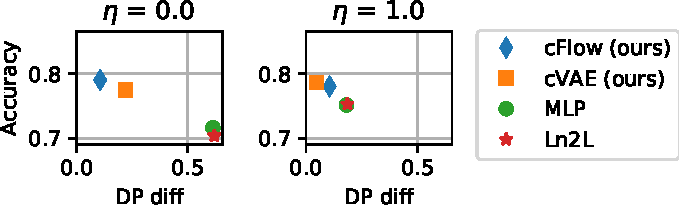
\includegraphics[width=0.6\textwidth]{nifr/Figures/nosinn_adult_multiplot_mini_diff.pdf}
  \caption{
      Results for the \textsc{Adult} dataset.
      The $x$-axis corresponds to the difference in positive rates.
      An ideal result would occupy the \textsc{top-left}.
  }%
  \label{fig:adult-chart}
\end{figure}
% \end{wrapfigure}

\paragraph{Results for the UCI Adult dataset.}
%
The UCI Adult dataset consists of census data and is commonly used to evaluate models focused on
\acl{AF}.
%
Following convention, we designate ``gender'' as the sensitive attribute $s$ and whether an
individual's salary is \$50,000 or greater as $y$.
%
We show the performance of our approach in comparison to baseline approaches in Fig.
\ref{fig:adult-chart}.
%
We evaluate the performance of all models for mixing factors ($\eta$) $0$ and $1$. 
%
Results shown in Fig. \ref{fig:adult-chart} show that we match or exceed the baseline.
%
In terms of fairness metrics, our approach generally outperforms the baseline models for both of
$\eta$.
%
Detailed results can be found in \S\ref{sec:additional-results}.

We also did experiments to show that the encoder transfers to other tasks. 
%
These transfer-learning experiments can be found in \S\ref{sec:transfer-learning}.

